\documentclass[12pt,a4paper]{article}

% ─── Page Layout ───────────────────────────────────────────────────────────────
\usepackage[a4paper, margin=0.8in, headheight=14pt]{geometry}

% ─── Fonts (XeLaTeX) ───────────────────────────────────────────────────────────
\usepackage{fontspec}
\usepackage{unicode-math}
\setmainfont{TeX Gyre Pagella}
\setmonofont[Scale=0.88]{TeX Gyre Cursor}
\setmathfont{Latin Modern Math}

% ─── Packages ──────────────────────────────────────────────────────────────────
\usepackage{xcolor}
\usepackage{colortbl}
\usepackage{titlesec}
\usepackage{enumitem}
\usepackage{tabularx}
\usepackage{booktabs}
\usepackage{array}
\usepackage{amsmath}
\usepackage{tikz}
\usetikzlibrary{shapes.geometric, arrows.meta, positioning, calc, fit, decorations.pathreplacing}
\usepackage{tcolorbox}
\tcbuselibrary{skins, breakable}
\usepackage{hyperref}
\usepackage{fancyhdr}
\usepackage{graphicx}
\usepackage{microtype}
\hyphenpenalty=10000
\exhyphenpenalty=10000
\sloppy
\usepackage{caption}
\usepackage{setspace}
\usepackage{multirow}
\usepackage{tocloft}

% ─── Q&A helper ────────────────────────────────────────────────────────────────
\newcommand{\Q}[1]{\textbf{#1}\par\noindent\ignorespaces}

% ─── Colour Palette ────────────────────────────────────────────────────────────
\definecolor{myred}{RGB}{196,30,58}
\definecolor{mydark}{RGB}{30,30,50}
\definecolor{mygreen}{RGB}{14,120,80}
\definecolor{myteal}{RGB}{0,130,140}
\definecolor{myamber}{RGB}{180,100,0}
\definecolor{mypurple}{RGB}{100,30,160}
\definecolor{mygray}{RGB}{246,247,249}
\definecolor{mgframe}{RGB}{180,185,200}
\definecolor{watermark}{RGB}{145,150,170}
\definecolor{hdrred}{RGB}{250,232,235}
\definecolor{hdrgreen}{RGB}{220,244,233}
\definecolor{hdrteal}{RGB}{220,242,244}
\definecolor{hdramber}{RGB}{253,242,215}
\definecolor{hdrpurple}{RGB}{238,228,255}
\definecolor{hdrgray}{RGB}{238,240,245}
\definecolor{rowalt}{RGB}{250,251,253}

% ─── Section Formatting ────────────────────────────────────────────────────────
\titleformat{\section}
  {\large\bfseries\color{myred}}{\thesection.}{0.5em}{}
  [\vspace{1pt}{\color{myred}\rule{\linewidth}{0.8pt}}]
\titleformat{\subsection}
  {\normalsize\bfseries\color{myteal}}{\thesubsection}{0.5em}{}
\titlespacing*{\section}{0pt}{18pt}{7pt}
\titlespacing*{\subsection}{0pt}{11pt}{4pt}

% ─── Paragraph ─────────────────────────────────────────────────────────────────
\setlength{\parindent}{0pt}
\setlength{\parskip}{4pt}

% ─── TOC Styling ───────────────────────────────────────────────────────────────
\renewcommand{\cfttoctitlefont}{\large\bfseries\color{myred}}
\renewcommand{\cftaftertoctitle}{\par\noindent{\color{myred}\rule{\linewidth}{0.8pt}}}
\setlength{\cftbeforetoctitleskip}{0pt}
\setlength{\cftaftertoctitleskip}{6pt}
\renewcommand{\cftsecfont}{\normalsize\bfseries\color{mydark}}
\renewcommand{\cftsecpagefont}{\normalsize\bfseries\color{mydark}}
\renewcommand{\cftsecleader}{\cftdotfill{\cftdotsep}}
\setlength{\cftbeforesecskip}{7pt}
\renewcommand{\cftsubsecfont}{\small\color{mydark}}
\renewcommand{\cftsubsecpagefont}{\small\color{mydark}}
\setlength{\cftbeforesubsecskip}{3pt}
\setlength{\cftsubsecindent}{1.4em}

% ─── Table helpers ─────────────────────────────────────────────────────────────
\renewcommand{\arraystretch}{1.45}
\setlength{\tabcolsep}{6pt}
\arrayrulecolor{mydark}
\newcolumntype{B}[1]{>{\small\bfseries\raggedright\arraybackslash}m{#1}}
\newcolumntype{Y}{>{\small\raggedright\arraybackslash}X}
\renewcommand{\tabularxcolumn}[1]{m{#1}}

% ─── Header / Footer ───────────────────────────────────────────────────────────
\pagestyle{fancy}
\fancyhf{}
\fancyhead[L]{\small\color{myred}\textbf{EC502}\;\color{mydark}--- Computer Architecture}
\fancyhead[R]{\small\color{myteal}\textbf{Module 3 Notes}}
\fancyfoot[C]{\small\color{mydark}\thepage}
\fancyfoot[R]{\small\color{watermark}\textit{\copyright\ Biraj}}
\renewcommand{\headrulewidth}{0.5pt}
\renewcommand{\footrulewidth}{0.3pt}

% ─── Hyperref ──────────────────────────────────────────────────────────────────
\hypersetup{
  colorlinks=true, linkcolor=myteal, urlcolor=myteal,
  pdfauthor={Biraj Sarkar},
  pdftitle={EC502 --- Module 3 Notes}
}

% ─── tcolorbox styles ──────────────────────────────────────────────────────────
\tcbset{
  tikzbox/.style={
    colback=mygray, colframe=mgframe, boxrule=0.6pt, arc=4pt,
    left=8pt, right=8pt, top=6pt, bottom=6pt,
    colbacktitle=mgframe, coltitle=mydark,
    fonttitle=\small\bfseries
  },
  defbox/.style={
    colback=hdrgreen, colframe=mygreen, boxrule=0.8pt, arc=4pt,
    left=9pt, right=9pt, top=6pt, bottom=6pt,
    colbacktitle=mygreen, coltitle=white,
    fonttitle=\small\bfseries
  },
  formulabox/.style={
    colback=hdrteal, colframe=myteal, boxrule=0.8pt, arc=4pt,
    left=9pt, right=9pt, top=7pt, bottom=7pt,
    colbacktitle=myteal, coltitle=white,
    fonttitle=\small\bfseries
  },
  examplebox/.style={
    colback=hdramber, colframe=myamber, boxrule=0.8pt, arc=4pt,
    left=9pt, right=9pt, top=6pt, bottom=6pt,
    colbacktitle=myamber, coltitle=white,
    fonttitle=\small\bfseries
  },
  masonbox/.style={
    colback=hdrpurple, colframe=mypurple, boxrule=0.8pt, arc=4pt,
    left=9pt, right=9pt, top=6pt, bottom=6pt,
    colbacktitle=mypurple, coltitle=white,
    fonttitle=\small\bfseries
  },
  exambox/.style={
    colback=hdrpurple, colframe=mypurple, boxrule=1pt, arc=5pt,
    left=10pt, right=10pt, top=8pt, bottom=8pt,
    colbacktitle=mypurple, coltitle=white,
    fonttitle=\bfseries,
    breakable, title after break={\textbf{Frequently Asked / Viva Questions (contd.)}}}
}
% Make all boxes breakable across pages
\tcbset{breakable}

% ─── TikZ styles ───────────────────────────────────────────────────────────────
\tikzset{
  block/.style={rectangle, draw=myteal, fill=hdrteal,
    text width=2.4cm, align=center, minimum height=0.95cm,
    font=\small, rounded corners=3pt, line width=0.7pt},
  redblock/.style={rectangle, draw=myred, fill=hdrred,
    text width=2.4cm, align=center, minimum height=0.95cm,
    font=\small, rounded corners=3pt, line width=0.7pt},
  netnode/.style={rectangle, draw=myteal, fill=hdrteal,
    text width=1.5cm, align=center, minimum height=0.8cm,
    font=\small, rounded corners=3pt, line width=0.7pt},
  sumjunc/.style={circle, draw=myamber, fill=hdramber,
    minimum size=0.62cm, font=\small, line width=0.8pt},
  snode/.style={circle, draw=mypurple, fill=hdrpurple,
    minimum size=0.55cm, font=\footnotesize, line width=0.7pt},
  arrow/.style={-Stealth, thick, color=mydark},
  redarrow/.style={-Stealth, thick, color=myred},
  line/.style={thick, color=mydark}
}

% ═══════════════════════════════════════════════════════════════════════════════
\begin{document}
% ═══════════════════════════════════════════════════════════════════════════════

\begin{center}
  {\LARGE\bfseries\color{myred} EC502 --- Computer Architecture}\\[5pt]
  {\normalsize\color{mydark} Semester V \quad$\bullet$\quad 3L:0T:0P \quad$\bullet$\quad 3 Credits}\\[3pt]
  {\normalsize\color{myteal}\textbf{Module 3 Exam Notes: Computer Arithmetic and ALU Design}}\\[3pt]
  {\small\color{mydark} CGEC \;$|$\; B.Tech ECE (2023--27) \;$|$\; \textit{Biraj Sarkar}}
\end{center}
\vspace{2pt}
\noindent{\color{myred}\rule{\linewidth}{1.5pt}}
\vspace{2pt}

\hypersetup{linkcolor=mydark}
\tableofcontents
\hypersetup{linkcolor=myteal}
\newpage

\section{Computer Arithmetic and ALU Design}
\begin{tcolorbox}[defbox,title={Arithmetic logic unit}]
An arithmetic logic unit (ALU) is a combinational circuit that performs selected arithmetic and bitwise operations. An operation field controls the result multiplexer, and flag logic describes the result for later instructions.
\end{tcolorbox}
\subsection{Full adder, ripple carry and carry look-ahead}
For bits $A_i,B_i$ and carry $C_i$, define propagate $P_i=A_i\oplus B_i$ and generate $G_i=A_iB_i$. Then $S_i=P_i\oplus C_i$ and $C_{i+1}=G_i+P_i C_i$, with $+$ denoting Boolean OR in these carry equations.
\begin{itemize}[leftmargin=*,itemsep=3pt]
\item \textbf{Ripple carry.} Chain the full adders. The worst-case carry delay grows with word length because the high stage waits for the low stages.
\item \textbf{Carry look-ahead (CLA).} Substitute the carry recurrence repeatedly. Generate intermediate carries in parallel using the input propagate and generate signals.
\end{itemize}
\[
\begin{aligned}
 C_1&=G_0+P_0C_0,\\
 C_2&=G_1+P_1G_0+P_1P_0C_0,\\
 C_3&=G_2+P_2G_1+P_2P_1G_0+P_2P_1P_0C_0,\\
 C_4&=G_3+P_3G_2+P_3P_2G_1+P_3P_2P_1G_0+P_3P_2P_1P_0C_0 .
\end{aligned}
\]
Define group propagate $P=P_3P_2P_1P_0$ and group generate $G$ as the four $C_4$ terms not multiplying $C_0$. Then $C_4=G+PC_0$. Large adders use groups or a carry tree to limit gate fan-in. The trade-off is extra logic and wiring.
\begin{tcolorbox}[examplebox,title={Trace a carry through a CLA group}]
For $A=\texttt{1011}$, $B=\texttt{0101}$ and $C_0=0$, $P=\texttt{1110}$ and $G=\texttt{0001}$ as bit vectors here. Bit zero generates a carry and the next three bits propagate it. $C_1=C_2=C_3=C_4=1$. The four-bit output is \texttt{0000} with carry out 1.
\end{tcolorbox}

\subsection{Add/subtract, logic and shift selection}
A shared $n$-bit adder uses input $B'_i=B_i\oplus\mathrm{SUB}$ and $C_0=\mathrm{SUB}$. With $\mathrm{SUB}=0$ it adds. With $\mathrm{SUB}=1$ it computes $A+\overline B+1=A-B$ modulo $2^n$.
\begin{tcolorbox}[tikzbox,title={Result selection in a small ALU},unbreakable]
\centering
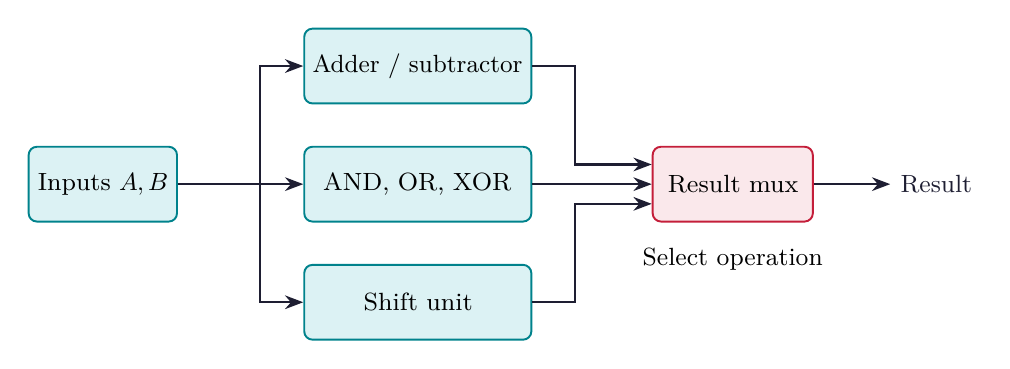
\begin{tikzpicture}[font=\small]
\node[block,text width=1.65cm] (in) at (0,0) {Inputs $A,B$};
\node[block,text width=2.65cm] (arith) at (4,1.5) {Adder / subtractor};
\node[block,text width=2.65cm] (logic) at (4,0) {AND, OR, XOR};
\node[block,text width=2.65cm] (shift) at (4,-1.5) {Shift unit};
\node[redblock,text width=1.8cm] (mux) at (8,0) {Result mux};
\draw[arrow] (in.east)--(2,0)|-(arith.west);
\draw[arrow] (in.east)--(logic.west);
\draw[arrow] (2,0)|-(shift.west);
\draw[arrow] (arith.east)--(6,1.5)|-($(mux.west)+(0,.25)$);
\draw[arrow] (logic.east)--(mux.west);
\draw[arrow] (shift.east)--(6,-1.5)|-($(mux.west)+(0,-.25)$);
\draw[arrow] (mux.east)--(10,0) node[right] {Result};
\node[below] at (8,-.69) {Select operation};
\end{tikzpicture}
\end{tcolorbox}

\begin{itemize}[leftmargin=*,itemsep=3pt]
\item \textbf{Flags.} $Z=1$ when all result bits are zero. $N$ copies the top bit. For add/subtract, carry comes from the top adder position, and signed overflow is the XOR of the carries into and out of that position.
\item \textbf{Shifts.} Logical right shift fills with zero. Arithmetic right shift replicates the sign. Rotate recirculates bits. A barrel shifter selects shifts by powers of two in successive mux stages.
\item \textbf{Compare.} A compare can compute a subtraction only for flags. For conventional two's-complement subtraction, signed less-than uses $N\oplus V$. Unsigned less-than uses borrow, accounted for by the selected carry convention.
\end{itemize}

\section{Binary Multiplication and Division}
\subsection{Unsigned shift-and-add multiplication}
Each bit of the multiplier selects a shifted copy of the multiplicand. For $M=13=\texttt{1101}$ and $Q=11=\texttt{1011}$, the selected copies are $13$, $13\cdot2$ and $13\cdot8$, giving 143 or \texttt{10001111}.
\begin{itemize}[leftmargin=*,itemsep=3pt]
\item \textbf{Sequential multiplier.} Put the multiplier in $Q$ and clear the high accumulator $A$. For each bit, conditionally add $M$ to $A$ when $Q_0=1$, then shift the carry and the joined $A:Q$ right. Keep the extra carry during the shift. After $n$ iterations, $A:Q$ holds the $2n$-bit product.
\item \textbf{Parallel multiplier.} An AND array generates partial products. Carry-save adders reduce rows to two without propagating carry across the entire width at every layer. A final carry-propagate adder adds the two rows. An array or tree costs more hardware than a reused sequential adder.
\end{itemize}

\subsection{Booth signed multiplication}
In radix-2 Booth multiplication, examine $(Q_0,Q_{-1})$, starting with $Q_{-1}=0$. The signed digit at bit $i$ is $q_{i-1}-q_i$. This replaces a run of ones from $i=l$ through $h$ by $2^{h+1}-2^l$ for a run that ends before the sign bit. The sign bit is handled by the same two's-complement recoding. Add $M$ for pair 01, subtract $M$ for 10, and do nothing for 00 or 11. Then arithmetic-right-shift $A:Q:Q_{-1}$ as one unit.
\begin{tcolorbox}[examplebox,title={Booth table for two negative numbers}]
Use $M=-6=\texttt{1010}$, $Q=-3=\texttt{1101}$ and $A=\texttt{0000}$. Use four iterations. The table shows registers after each arithmetic shift.
\par\vspace{6pt}\noindent
\begin{tabularx}{\linewidth}{|B{1.0cm}|B{1.2cm}|Y|B{1.7cm}|B{1.7cm}|B{1.2cm}|}\hline
Step & Pair & Operation before shift & $A$ & $Q$ & $Q_{-1}$ \\ \hline
1 & 10 & $A\leftarrow A-M$ & \texttt{0011} & \texttt{0110} & 1 \\ \hline
2 & 01 & $A\leftarrow A+M$ & \texttt{1110} & \texttt{1011} & 0 \\ \hline
3 & 10 & $A\leftarrow A-M$ & \texttt{0010} & \texttt{0101} & 1 \\ \hline
4 & 11 & No addition & \texttt{0001} & \texttt{0010} & 1 \\ \hline
\end{tabularx}

The joined result is \texttt{00010010}, or $+18$. For a fully general $n$-bit implementation use an extra sign bit in $A$ and sign-extend $M$ before add/subtract, then retain the low $2n$ product bits. This avoids overflow when negating the most negative multiplicand.
\end{tcolorbox}

\subsection{Restoring and non-restoring division}
\begin{tcolorbox}[defbox,title={Division invariant}]
For unsigned dividend $D$ and positive divisor $M$, return quotient $Q$ and remainder $R$ satisfying $D=MQ+R$ and $0\le R<M$. A zero divisor must be detected separately.
\end{tcolorbox}

In register division, initialise $A=0$ and $Q=D$. Repeat $n$ times for an $n$-bit dividend. $A$ is the signed partial remainder and needs enough extra width for the shift and trial addition/subtraction.
\begin{itemize}[leftmargin=*,itemsep=3pt]
\item \textbf{Restoring.} Shift $A:Q$ left, then subtract $M$ from $A$. If the trial is negative, set $Q_0=0$ and add $M$ back. Otherwise set $Q_0=1$.
\item \textbf{Non-restoring.} Remember the sign of $A$ before shift. Shift $A:Q$ left, subtract $M$ if the old sign was nonnegative, otherwise add $M$. Set $Q_0$ to 1 iff the new $A$ is nonnegative. At the end add $M$ once if $A<0$.
\item \textbf{Why the addition works.} If a trial is $A_{\rm trial}=a-M<0$, restoring then taking the next trial with incoming bit $b$ would give $2a+b-M$. Non-restoring obtains the same quantity as $2(a-M)+b+M$.
\end{itemize}
\begin{tcolorbox}[examplebox,title={Restoring and non-restoring traces for 13 divided by 3}]
Use $Q=\texttt{1101}$ and $M=3$. The quotient register in the last column is common to both runs at each step.
\par\vspace{6pt}\noindent
\begin{tabularx}{\linewidth}{|B{1.1cm}|Y|Y|Y|B{1.6cm}|}\hline
Step & Restoring trial & After restoration if needed & Non-restoring new $A$ & $Q$ \\ \hline
1 & $-2$ & $1$ & $-2$ & \texttt{1010} \\ \hline
2 & $0$ & $0$ & $0$ & \texttt{0101} \\ \hline
3 & $-3$ & $0$ & $-3$ & \texttt{1010} \\ \hline
4 & $-2$ & $1$ & $-2$ & \texttt{0100} \\ \hline
\end{tabularx}

The non-restoring method corrects $-2$ to $1$ at the end. In each case $Q=4$, $R=1$, and $13=3(4)+1$. Signed division can divide magnitudes and then apply the quotient and remainder sign convention. A minimum signed integer divided by $-1$ can overflow at fixed width.
\end{tcolorbox}

\section{IEEE 754 Formats and Floating-Point Arithmetic}
\subsection{Stored fields and special cases}
\begin{tcolorbox}[defbox,title={Binary floating-point format}]
An IEEE 754 binary interchange value uses a sign bit $s$, a biased exponent field $e$, and a fraction field of $p$ bits. Interpret the fields using the exponent class before applying the value formula.
\end{tcolorbox}
\par\vspace{6pt}\noindent
\begin{tabularx}{\linewidth}{|B{3cm}|Y|Y|Y|}\hline
Format & Sign / exponent / fraction & Bias & Normal precision \\ \hline
Binary32 & $1/8/23$ & $127$ & $24$ bits \\ \hline
Binary64 & $1/11/52$ & $1023$ & $53$ bits \\ \hline
\end{tabularx}

Let $F$ be the unsigned integer encoded by the fraction bits and $f=F/2^p$. With all-ones exponent denoted $e_{\max}$:
\begin{itemize}[leftmargin=*,itemsep=3pt]
\item \textbf{Normal} ($0<e<e_{\max}$): $(-1)^s(1+f)2^{e-\mathrm{bias}}$. The leading 1 is implicit.
\item \textbf{Subnormal} ($e=0,\ F\ne0$): $(-1)^s f2^{1-\mathrm{bias}}$. The hidden bit is 0. Smallest positive binary32 normal is $2^{-126}$ and smallest subnormal is $2^{-149}$.
\item \textbf{Signed zero} ($e=0,\ F=0$): $\pm0$. \textbf{Infinity} ($e=e_{\max},\ F=0$): $\pm\infty$. \textbf{NaN} ($e=e_{\max},\ F\ne0$): not a number, as can result from $0/0$.
\end{itemize}
\begin{tcolorbox}[examplebox,title={Encode negative 13.25 in binary32}]
Magnitude $13.25=1101.01_2=1.10101_2\times2^3$. Set $s=1$ and $e=3+127=130=\texttt{10000010}$. Store fraction bits \texttt{10101} followed by 18 zeros. Concatenating fields gives hexadecimal \texttt{C1540000}. To decode it, restore the leading 1, subtract the bias and apply the sign.
\end{tcolorbox}

\subsection{Addition, subtraction, multiplication and division}
\begin{enumerate}[leftmargin=*,itemsep=3pt]
\item \textbf{Unpack and classify.} Separate signs, exponents and significands. Handle zeros, infinities and NaNs as specified before using normal-number formulas.
\item \textbf{Add or subtract.} Align exponents by shifting the smaller-exponent significand right. Add or subtract according to the signs. Normalise the result and update the exponent. Cancellation may require left shifts. Example:
\[
 (1.101_2\times2^3)+(1.1_2\times2^0)
 =(1.101_2+0.0011_2)2^3=1.1101_2\times2^3 .
\]
\item \textbf{Multiply or divide.} XOR the signs. Multiply significands and add unbiased exponents, or divide significands and subtract unbiased exponents. Normalise afterwards. For multiplication, $(1.1_2\times2^0)(1.1_2\times2^{-1})=10.01_2\times2^{-1}=1.001_2\times2^0$.
\item \textbf{Round and pack.} Round to the target precision and range, then pack the fields. Rounding can create a new carry and change the exponent.
\end{enumerate}
\begin{tcolorbox}[examplebox,title={Normalise after subtraction and division}]
\[
\begin{aligned}
(1.010_2-1.001_2)2^2
 &=0.001_2\times2^2=1.000_2\times2^{-1},\\
\frac{1.001_2\times2^3}{1.1_2\times2^1}
 &=0.11_2\times2^2=1.1_2\times2^1 .
\end{aligned}
\]
The subtraction cancels leading bits and requires three left shifts. The division yields a significand below one and requires one left shift. Decrease the exponent once per left shift.
\end{tcolorbox}

\subsection{Rounding and exceptions}
\begin{itemize}[leftmargin=*,itemsep=3pt]
\item \textbf{Guard, round and sticky.} The first two extra bits are guard and round. Sticky is the OR of the remaining discarded bits.
\item \textbf{Nearest, ties-to-even.} Increment the retained significand if guard is 1 and any of round, sticky or the last retained bit is 1. At a midpoint select the even last bit. With three fraction bits, $1.0101000_2$ rounds to $1.010_2$ and $1.0111000_2$ rounds to $1.100_2$.
\item \textbf{Other rounding directions.} Directed modes can round toward zero, $+\infty$ or $-\infty$.
\item \textbf{Status conditions.} Invalid operation, division by zero, overflow, underflow and inexact result are distinct. Overflow handling depends on the rounding direction. Subnormals allow gradual underflow. An exactly representable subnormal does not by itself imply inexact underflow.
\end{itemize}

\newpage
\begin{center}
  {\large\bfseries\color{myred} Quick Revision --- Module 3}\\[3pt]
  {\small\color{mydark} Computer Arithmetic and ALU Design $|$ EC502}
\end{center}
\noindent{\color{myred}\rule{\linewidth}{1.2pt}}
\begin{tcolorbox}[formulabox,title={Key Formulas at a Glance}]
\renewcommand{\arraystretch}{1.35}
\begin{tabularx}{\linewidth}{B{5.0cm}Y}
Full-adder carry & $C_{i+1}=G_i+P_i C_i$ \\[3pt]
Shared add/subtract & $B'=B\oplus\mathrm{SUB}$ and $C_0=\mathrm{SUB}$ \\[3pt]
Booth pair rule & 01 adds, 10 subtracts, 00 and 11 hold \\[3pt]
Unsigned division & $D=MQ+R$ with $0\le R<M$ \\[3pt]
IEEE normal & $(-1)^s(1+f)2^{e-\mathrm{bias}}$ \\[3pt]
IEEE subnormal & $(-1)^sf2^{1-\mathrm{bias}}$ \\[3pt]
\end{tabularx}
\end{tcolorbox}
\begin{tcolorbox}[defbox,title={One-Line Definitions}]
\textbf{Generate bit.} Indicates an output carry independent of the incoming carry.\par
\textbf{Sticky bit.} OR of the bits discarded beyond the round bit.\par
\textbf{Subnormal.} Nonzero floating-point value with a zero exponent field and an implicit leading zero.\par
\end{tcolorbox}
\begin{tcolorbox}[exambox,title={Frequently Asked / Viva Questions}]
\begin{enumerate}[topsep=0pt, label=\textbf{Q\arabic*.}, itemsep=5pt]
\item \Q{Why is ripple carry slow at large widths?}
A carry may propagate through all stages.
\item \Q{Why does subtract set carry-in to one?}
It completes the two's complement of the second operand.
\item \Q{How many product bits suffice for two n-bit inputs?}
A full-width product uses $2n$ bits.
\item \Q{Which shift follows each Booth action?}
An arithmetic right shift of the joined accumulator, multiplier and saved bit.
\item \Q{What is restored in restoring division?}
A negative trial partial remainder is returned to its value before subtraction.
\item \Q{What is the final correction in non-restoring division?}
Add the divisor once if the final remainder is negative.
\item \Q{Why align exponents before floating-point addition?}
Significands must use the same power-of-two scale.
\item \Q{How many stored fraction bits does binary64 use?}
52, giving 53 bits of normal precision.
\item \Q{What distinguishes infinity from NaN?}
With all-ones exponent, infinity has zero fraction and NaN has nonzero fraction.
\item \Q{What does ties-to-even do at an exact midpoint?}
Selects the result whose last retained significand bit is zero.
\end{enumerate}
\end{tcolorbox}
\begin{tcolorbox}[tikzbox,title={Summary comparison}]
\begin{tabularx}{\linewidth}{|B{4cm}|Y|}\hline
\textbf{Case} & \textbf{What to use} \\ \hline
Ripple / CLA & Serial carry propagation / parallel group carry equations. \\ \hline
Restoring / non-restoring & Correct negative trials immediately / compensate in the next cycle and correct at the end. \\ \hline
Normal / subnormal & Implicit leading one / implicit leading zero. \\ \hline
\end{tabularx}
\end{tcolorbox}
\end{document}
